\documentclass[../main.tex]{subfiles}

\begin{document}

\section{Configuración del entorno de programación}

    Las prácticas de la asignatura de PSyD se desarrollan en un entorno ya preparado dentro de una máquina virtual. Esto es debido a la comodidad y portabilidad que ofrece, ya que con trasladar un simple fichero, cualquiera puede tener todas las herramientas disponibles en su ordenador. No obstante, también se ofrece aquí una guía de instalación para quien quiera instalarlo todo de manera nativa en su ordenador. La guía se ha realizado para Ubuntu. Su adaptación a otros sistemas operativos (MacOS, o Windows) es relativamente directa, al estar las herramientas disponibles para todas las plataformas. 

    \subsection{Configuración para máquina virtual}\label{sub:vmconfig}
        El software y los recursos necesarios ya están preinstalados en una máquina virtual basada en \textbf{Debian 13.6}. Cuenta con un entorno ligero (gestor de ventanas, navegador básico) y las \textbf{VirtualBox Guest Additions} para habilitar el passthrough de dispositivos USB (necesario para conectar la placa).

        Puedes descargar la máquina virtual ya configurada y lista para importar en VirtualBox desde \url{https://drive.google.com/file/d/1U7Qvnkb-LfkJrcboyH4Jzs9iNczMntQg/view?usp=drivesdk}. También es necesario descargar \textbf{VirtualBox} para arrancarla. Para ello sigue las siguientes instrucciones:

        \begin{itemize}
            \item Asegúrate de tener instalado \textbf{VirtualBox} en su versión más reciente. Puedes descargarlo desde \url{https://www.virtualbox.org/wiki/Downloads}.
            \item Importante también descargar, desde el mismo enlace, el ``VirtualBox Extension Pack''. Sin él, perderemos funcionalidades de la MV, entre otros, la capacidad de conectarle USBs (como el depurador ST-Link de la placa).
        \end{itemize}

    \subsection{Creación de la Máquina Virtual}
        Sigue esta parte sólo si quieres crear una máquina virtual propia desde cero. Si quieres hacerlo de manera nativa, salta a \Cref{sub:toolkitsetup}.

        Crea una nueva máquina virtual e instala \textbf{Debian} en su última versión (\url{https://www.debian.org/index.es.html}) o \textbf{Ubuntu} (recomendado versión \textbf{24.04 LTS}, descargable desde \url{https://ubuntu.com/download}). Configura el hardware asignándole los siguientes recursos recomendados:
        \begin{itemize}
            \item \textbf{Memoria RAM:} 4096 MB
            \item \textbf{Procesadores:} 2 núcleos (Cores).
            \item \textbf{Memoria de Vídeo:} 128 MB.
            \item \textbf{Tamaño del disco:} 60GB.
            \item \textbf{Tipo de instalación:} Manual. No utilizar la automática ya que instala cosas de más.
        \end{itemize}

        Una vez seleccionados los recursos, lanza la máquina y el instalador comenzará automáticamente. Deberás seleccionar cuestiones como el nombre de la máquina, usuario, contraseña... elige el que más te guste. El resto de la configuración se puede dejar por defecto. Ten en cuenta que el proceso de instalación puede tardar una una media hora (dependiendo del sistema anfitrión). Se recomienda utilizar las instalaciones gráficas para tener todo el sistema operativo bien preconfigurado. No obstante, también se pueden hacer instalaciones manuales para ajustar mejor las herramientas disponibles y, con ello, el tamaño de la máquina.

        Una vez arranque la máquina, es importante instalar los extras de invitado (``Guest additions''), para conseguir que anfitrión y host se comunique adecuadamente (y puedan por ejemplo compartir portapapeles, ajustar el tamaño de pantalla, etc). Para ello haz click en \texttt{devices > insert guest additions CD image}. Esto cargará un disco en la MV (panel izquierdo). Abre una terminal en la ruta donde se monta el CD (normalmente /media/cdrom) y ejecuta:

        \begin{lstlisting}
        # Actualizar paquetes existentes
        > sudo apt update && sudo apt upgrade
        # Instalar herramientas para compilar las guest additions
        > sudo apt install build-essential dkms linux-headers-$
        # Instalar guest additions
        > sudo ./VBoxLinuxAdditions.run
        \end{lstlisting}


    \subsection{Configuración del ToolKit de STM}\label{sub:toolkitsetup}
        Independientemente de si quieres utilizar tu propio sistema operativo para instalar las herramientas, o instalarlas en la máquina virtual, se hace de la misma manera. A continuación se muestran todas las herramientas, repositorios, etc necesarios para tener todo lo necesario en la asignatura. Si prefieres no realizar la instalación, descarga la máquina virtual ya configurada como se indica en el primer paso (\Cref{sub:vmconfig}).

        \begin{itemize}
            \item Instalar STM32CubeIDE (la herramienta principal de desarrollo) desde aquí: \url{https://www.st.com/en/development-tools/stm32cubeide.html}
            \item Instalar STM32CubeMX (para configuración avanzada) desde aquí: \url{https://www.st.com/en/development-tools/stm32cubemx.html}
            \item Instalar STM32CubeProgrammer (para compatibilidad con zephyr) desde aquí: \url{https://www.st.com/en/development-tools/stm32cubeprog.html}
            \item Instalar picocom para comunicar con la placa con posterioridad:
                \begin{lstlisting}
                    > sudo apt-get install picocom
                \end{lstlisting}
        \end{itemize}

    \subsection{Descarga de manuales y recursos extra}
        Dentro de la MV ya creada, en la carpeta \textbf{Documentos} del entorno se encuentran varios recursos en forma de manuales. Si se está haciendo la instalación manual, estos son los recursos que ahí se encuentran y haría falta descargar:

        \begin{itemize}
            \item \REFMAN : \url{https://www.st.com/resource/en/reference_manual/rm0431-stm32f72xxx-and-stm32f73xxx-advanced-armbased-32bit-mcus-stmicroelectronics.pdf}
            
                Manual principal de referencia. Detalla toda la funcionalidad de los procesadores de la serie \textbf{STM32F723}, incluyendo periféricos, mapa de memoria, registros, modos de uso, etc.

            \item \BRDMAN : \url{https://www.st.com/resource/en/user_manual/um2140-discovery-kit-with-stm32f723ie-mcu-stmicroelectronics.pdf}
            
                Manual con la descripción de conexiones y \textit{pinout} detallado del kit de desarrollo \BOARD.

            \item \DSMAN : \url{https://www.st.com/resource/en/datasheet/stm32f722ic.pdf}

                Funcionalidad genérica, especificaciones físicas y características electrónicas del procesador \MCU.
            
            \item \PMMAN : \url{https://www.st.com/resource/en/programming_manual/pm0253-stm32f7-series-and-stm32h7-series-cortexm7-processor-programming-manual-stmicroelectronics.pdf}
            
                Manual de programación de la serie \textbf{Cortex-M7}, con la referencia completa del conjunto de instrucciones ensamblador.

            \item \LCDMAN : \url{https://www.crystalfontz.com/controllers/Sitronix/ST7789H2}
            
                Manual de características del panel LCD \texttt{ST7789H2} integrado en la placa.
            
            \item \ANMAN : \url{https://www.st.com/resource/en/application_note/cd00167594-stm32-microcontroller-system-memory-boot-mode-stmicroelectronics.pdf}
            
                Manual sobre las secuencias de inicialización (\emph{bootloading}) en los dispositivos de ST.

            \item \textbf{DB3105}: \url{https://www.st.com/resource/en/data_brief/32f723ediscovery.pdf}

                Resumen de características del kit de desarrollo \BOARD.    
        \end{itemize}

        Adicionalmente, también se incluye en la MV creada la colección de ejemplos oficiales \textbf{STM32CubeF7}.

        \textbf{Nota:} Esta colección utiliza librerías de alto nivel (HAL/LL). En la primera parte de las prácticas programaremos ``desde cero'' (a nivel de registro), por lo que no usaremos estas librerías directamente. Sin embargo, los ejemplos son un buen punto de referencia para explorar las capacidades de la placa.

        \begin{itemize}
            \item \textbf{STM32CubeF7 (GitHub)} \url{https://github.com/STMicroelectronics/STM32Cubef7}
                    
                Colección de ejemplos base. Incluye proyectos para múltiples placas, pero nos centraremos únicamente en la \BOARD. 

                Al clonar manualmente el repositorio, es imprescindible inicializar los submódulos para incluir todas las librerías requeridas. Mira bien las instrucciones del repositorio.

            \item \textbf{STM32CubeF7 Patch} \url{https://www.st.com/en/embedded-software/stm32cubef7.html}

                Parche que se debe sobrescribir en el repositorio una vez clonado. Añade librerías propietarias de terceros necesarias para funciones como el control táctil o el procesamiento de audio.
        \end{itemize}

    \subsection{Descarga del material de la asignatura}

        El material de la asignatura se encuentra completo en \url{https://github.com/Daniel-BG/PSyD}, incluyendo teoría, práctica y códigos de ejemplo. Se recomienda descargarlo entero mediante la herramienta de terminal \texttt{git} (o cualquier otra herramienta que permita descargar repositorios). Desde la terminal de la máquina virtual (o la terminal nativa de tu ordenador), ejecuta:

        \begin{lstlisting}
            > git clone https://github.com/Daniel-BG/PSyD
        \end{lstlisting}

        \textbf{NOTA:} Si la herramienta \texttt{git} no estuviera disponible, en linux se puede instalar con:

        \begin{lstlisting}
            >  sudo apt-get install git
        \end{lstlisting}

        Se descargará y creará una carpeta llamada \texttt{PSyD}, con los siguientes contenidos:

        \definecolor{doccomment}{rgb}{0.4, 0.8, 0.4}
        \newcommand{\grcomment}[1]{\DTcomment{\textcolor{doccomment}{-- #1}}}

        \dirtree{%
            .1 code/\grcomment{Código fuente de las prácticas}.
                .2 ws\_desarrollo/\grcomment{Proyectos SIN solución (punto de partida)}.
                    .3 <nombre\_practica>/\grcomment{Ficheros de proyecto STM32/CubeIDE}.
                .2 ws\_soluciones/\grcomment{Proyectos CON solución (para consulta)}.
                    .3 <nombre\_practica>/\grcomment{Misma estructura resuelta}.
            .1 practicas/\grcomment{Enunciados y documentación}.
                .2 main.\{pdf,tex\}\grcomment{Compilación completa de prácticas}.
                .2 practicas.md\grcomment{Información general}.
                .2 <nombre\_practica>/\grcomment{Carpeta individual por práctica}.
                    .3 <nombre\_practica>.\{pdf,tex\}\grcomment{Enunciado en fuente y renderizado}.
                    .3 res/\grcomment{Recursos gráficos e imágenes}.
            .1 teoria/\grcomment{Material teórico}.
                .2 main.\{pdf,tex\}\grcomment{Libro/Documento completo de teoría}.
                .2 <capitulo>/\grcomment{Capítulo individual}.
                    .3 <capitulo>.\{pdf,tex\}\grcomment{Fuente y PDF del capítulo}.
        }

        Ahora, abriendo la herramienta STM32CubeIDE, podremos importar los proyectos. En primer lugar debemos establecer como \emph{workspace} la carpeta donde tenemos los códigos. Por ejemplo vamos a hacerlo con \texttt{ws\_desarrollo}, como se ve en la \Cref{fig:ws_import}.

        \begin{figure}
            \centering
            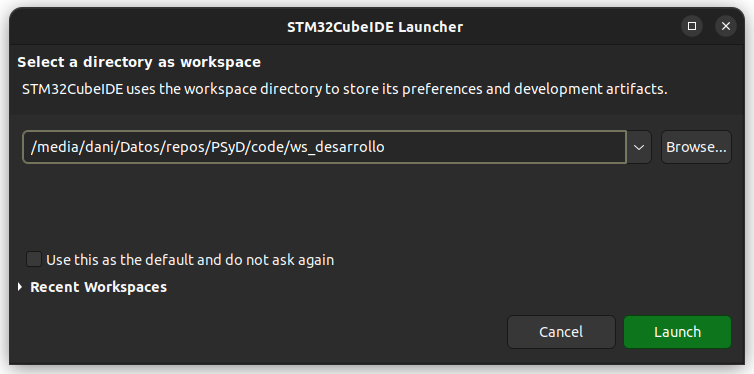
\includegraphics[width=0.6\textwidth]{res/ws_import.png}
            \caption{Elección de la carpeta para importar}
            \label{fig:ws_import}
        \end{figure}

        A continuación, haremos click en \texttt{file > STM32 Project create/import} para abrir la herramienta de importación, seleccionándola desde el menú que se abre (\Cref{fig:import_project}).

        \begin{figure}
            \centering
            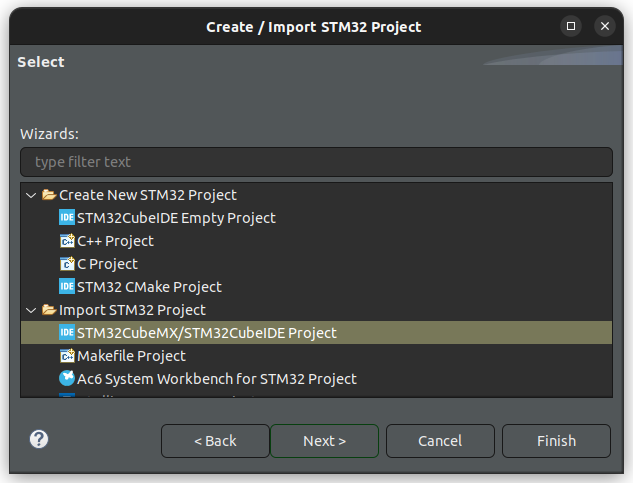
\includegraphics[width=0.6\textwidth]{res/import_project.png}
            \caption{Elegir importación de proyectos}
            \label{fig:import_project}
        \end{figure}

        Finalmente, buscamos de nuevo la carpeta del workspace (que es donde están los proyectos) y la elegimos en el menú. Esto nos mostrará los proyectos, y podemos elegir cuáles importar (si alguno no se importa ahora, se puede hacer más tarde). Ver la \Cref{fig:import_dialog}.

        \begin{figure}
            \centering
            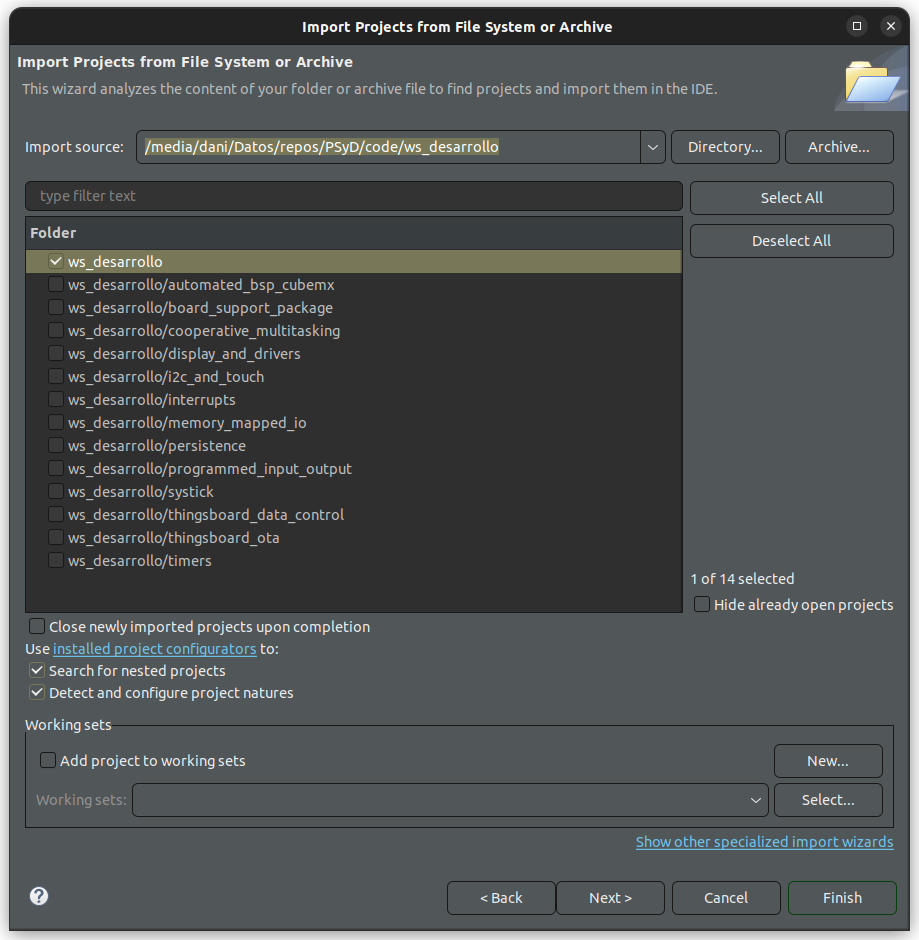
\includegraphics[width=\textwidth]{res/import_dialog.png}
            \caption{Elegir importación de proyectos}
            \label{fig:import_dialog}
        \end{figure}

        Tras importar los proyectos, los deberíamos ver en el panel lateral de la herramienta, ver \Cref{fig:after_import}.

        \begin{figure}
            \centering
            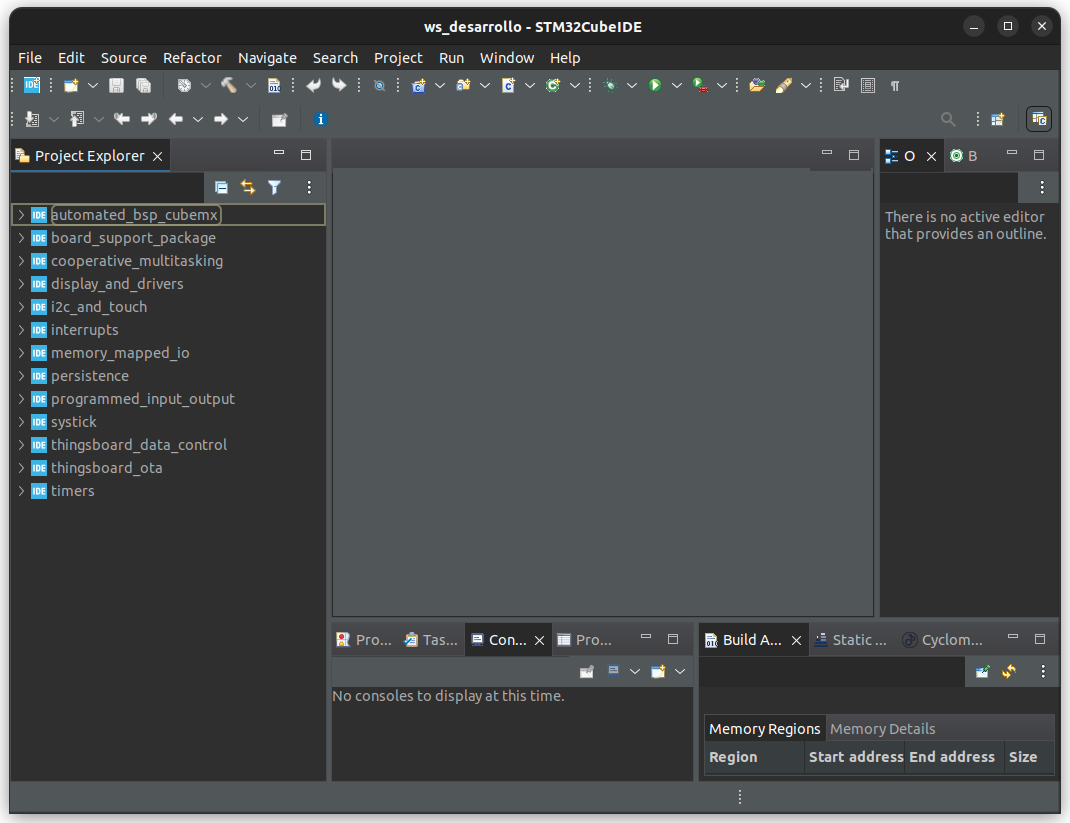
\includegraphics[width=\textwidth]{res/after_import.png}
            \caption{Elegir importación de proyectos}
            \label{fig:after_import}
        \end{figure}
    
    \subsection{Conexión de la placa a la máquina virtual}

        Si utilizas tu ordenador con STM32CubeIDE instalado nativamente, la placa debería detectarse automáticamente por el programa. Si usas la máquina virtual, hace falta indicarle al ordenador que pase el control del USB del sistema operativo anfitrión (el vuestro) al huésped (la máquina virtual). Para ello, con la máquina virtual ya abierta, seleccionar en el menú \texttt{devices > USB > ST-LINK} y activarlo.


\end{document}



%    \subsection{Paso 4: Configuración de las herramientas de Zephyr}
%        Para poder utilizar las herramientas de Zephyr, y compilar el sistema operativo en tiempo real para las placas, hay que hacer una serie de configuraciones relativamente complejas, que incluyen la descarga de varios repositorios. Aquí están las instrucciones oficiales, que replicamos en este documento: \url{https://docs.zephyrproject.org/latest/develop/getting_started/index.html#getting-started}.
%
%        \begin{lstlisting}
%            # Instala las dependencias necesarias para trabajar con zephyr:
%            > sudo apt install --no-install-recommends git cmake ninja-build \ 
%                gperf ccache dfu-util device-tree-compiler wget python3-dev \ 
%                python3-venv python3-tk xz-utils file make gcc gcc-multilib \ 
%                g++-multilib libsdl2-dev libmagic1
%            # Crea una carpeta para el \textbf{32F723EDISCOVERY}paquete de zephyr:
%            > mkdir ~/zephyrproject
%            # Crea un entorno virtual de python
%            > python3 -m venv ~/zephyrproject/.venv
%            # Cambia al entorno virtual para activar los paquetes de python necesarios
%            > source ~/zephyrproject/.venv/bin/activate
%            # Instala West (gestor de dependencias) e inicializa el proyecto
%            > pip install west
%            > west init -m https://github.com/zephyrproject-rtos/zephyr ~/zephyrproject
%            > cd ~/zephyrproject
%            > west update
%            # Exporta zephyr para que sea encontrado por otras herramientas
%            > west zephyr-export
%            # Instala las dependencias:
%            > west packages pip --install
%            # Instala el SDK de zephyr:
%            > cd ~/zephyrproject/zephyr
%            > west sdk install #(Usar primero --help para poner solo la toolchain de st)
%        \end{lstlisting}
%
%        Ya estamos listos para probar zephyr con un ejemplo y ver que funciona:
%        
%        \begin{lstlisting}
%            # Copy the blinky sample to a new folder
%            > cp -r zephyr/samples/basic/blinky my_blinky
%            > cd my_blinky
%            > west build -b stm32f412g_disco
%            (otra terminal) > picocom /dev/ttyACM0 -b 115200 -d 7 -p o
%            > west flash
%        \end{lstlisting}